\chapter{Implementation}
\section{Video Preprocessing}
Surveillance footage is usually generated of size 240 x 320 i.e of aspect ratio of 3:4. Considered video format is of avi. If the video is not present in the given format, we use the ffmpeg command to convert the video to the required format. 
\\
Video conversion command:-\\
\textit{ffmpeg -i {inputVideo} -vf scale=320:240 outputVideo.avi}
\par
Further the frame is resized to 75 x 100 size maintaining the same aspect ratio using openCV functions. This resized frame is further converted to grayscale using openCV cvtColor method. \\
Size reduction command:\\
frame = cv2.resize(frame, dim, interpolation = cv2.INTER\_AREA)\\
Grayscale conversion commands: \\
frame = cv2.cvtColor(frame,cv2.COLOR\_BGR2GRAY)
\begin{center}
\begin{figure}[H]
\centering
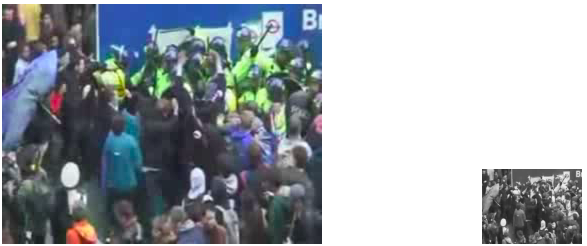
\includegraphics[width = \linewidth]{frame_resize.png}
\caption{Frames before and after preprocessing respectively}
\end{figure}
\end{center}
\section{Optical Flow}
Optical Flow is estimated between the pair of consecutive frames which gives a flow vector for each pixel in the current frame, matching it to pixel in next frame. C. Liu’s Optical Flow algorithm is used. It was initially developed in C++ which MATLAB can easily port. Conda package was used to port the algorithm into Python. \par
	In our implementation we are considering two frames in every four frames i.e the third frame from current frame and calculating optical flow between them. This process continues for entire video. \par \textbf{bob.ip.optflow.liu.sor.flow(frame1,frame2)} is used to calculate optical flow. It returns value of each pixel into a numpy array of dimension equal to resolution of the frame.
\begin{center}
\begin{figure}[H]
\centering
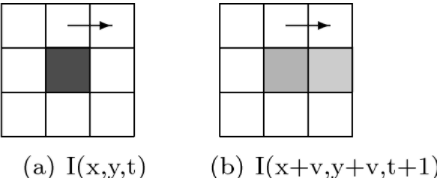
\includegraphics[width = \linewidth]{optical_flow.png}
\caption{Example Optical Flow}
\end{figure}
\end{center}

\section{Violent Features}
Once the optical flow has been generated, flow vector magnitude is calculated through the following formula:- \\
$ m_{x,y,t} = \sqrt{V_{x,t}^2 + V_{y,t}^2} $ \\
\par
After calculating flow vector , for each pixel in each frame we obtain the binary indicators using the following formula:- \\
\begin{equation}
b_{x,y,t} = \begin{cases}
\text {1,\quad}if\quad |m_{x,y,t+1} - m_{x,y,t-1}| \geq \theta\\
\text {0\quad}   \quad otherwise
\end{cases}
\end{equation}
\par
Next we calculate the mean magnitude change by simply averaging these binary indicators for each frame:- 
\begin{equation}
\overline b_{x,y} = \frac{1}{T}\sum_{t}b_{x,y,t}
\end{equation}
\par
This average binary vector obtained is known as Violent Flow Descriptor (ViF). This ViF values is used for further training and classifications purposes.
	After ViF’s are obtained for a video, a histogram in created of bin size 0.05 and from range 0.0 to 1.0. Which means 21 bins are created. Generated ViF is divided into 16 parts, each part is mapped into a separate histogram, the counts are further normalized by total counts obtained. This process is known as Histogram normalization. Now all these histogram bins values for all 16 parts are appended one after the other leading to generation 336 values for a particular video. 
These 336 values are used for training the neural net and for predicting using the neural net.
\section{Training Neural Net}
Keras module along with TensorFlow backend is used to build the Neural Net and Train it. The Neural Net built contains an Input Layer, two Dense Layers and an Output Layer. Each layer is of 336 nodes. Input to the neural net will the Violent Flow Features(ViF) which is a numpy array of dimensions 129*336. Activation function for Input and Middle Layers is ReLU(Rectifier Linear Unit) and for output layer, Sigmoid activation function is used. Training is done for 150 epochs with batch size of 10. Outputs will in the range of 0.0 to 1.0 which will rounded off accordingly. \\
ReLU activation Function \\
f(x) = max(0,x)\\
Sigmoid activation function \\
S(x) = $\frac{1}{1+e^{-x}} = \frac{e^x}{1+e^x}$
\begin{center}
\begin{figure}[H]
\centering
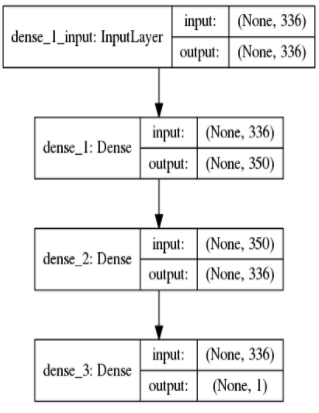
\includegraphics[scale = 0.6]{neural_net.png}
\caption{Neural Net Layer Information}
\end{figure}
\end{center}
\section{Violence Detection}
Keras module has been used to train the neural network. The average FPS rate of a video is to be considered 30fps. Average surveillance videos have an FPS rate of 30fps. We consider every 3rd frame for calculating ViF’s. 
\par
	Every 30 frames , i.e every 1 second 336 length array is generated and that array is sent to the previously generated model for prediction. If violence is detected, violence probability is shown on the screen. Multiple lengthy videos have been given an input to the program and it is able to detect the instance where crowd behaviour tends to violent from non\_violent.


